\subsubsection{Алгоритм}

Предварительного заполнения базы данных не требуется, однако для возможности добавления записи и регистрации пациента администратору сначала необходимо заполнить базу сотрудников и расписаний.

\begin{center}
  Шаг 1
\end{center}

При авторизации от имени пациента в главном окне программы (MainWindow) появится окно для записи на прием к врачу (EnrollWindow). Необходимо выбрать нужного специалиста, найти его расписание и правильно заполнить предлагаемую форму. Если входные значения были введены неверно, появится сообщение об ошибке. 

\begin{center}
  Шаг 2
\end{center}

Программа проверяет, есть ли уже в БД введенные пользователем серия и номер паспорта. Если данные о пациенте в базе уже есть и форма заполнена верно, появится сообщение об успешной записи, либо сообщение об ошибке записи, если такая запись уже была добавлена в БД.

\begin{center}
  Шаг 3
\end{center}

Если данных о пациенте в базе нет, то появится форма регистрации пациента (PatientRegisterWindow). Если все поля формы заполнены верно, пациент будет добавлен в базу и в окне записи на прием при повторной операции записи появится уведомление об успешном завершении операции, в результате которой будет сгенерирован PDF-файл (талон), готовый к печати.

\begin{center}
  Шаг 4
\end{center}

При авторизации от имени администратора программа сверяет хеш введённого пароля с  хешем, который хранится в БД. Если они совпадают, то открывается окно управления базой данных (AdminWindow), если нет, то появляется уведомление об ошибочной авторизации.

\begin{center}
  Шаг 5
\end{center}

Окно управления базой данных (AdminWindow) позволяет администратору просматривать, удалять и добавлять данные в базу. Для этого необходимо вводить корректные данные, в противном случае операции удаления и добавления выполняться не будут, появится сообщение об ошибке ввода или обращения к базе.

Блок-схема алгоритма работы программы представлена на рисунке~\ref{block:block}.

\begin{figure}[h!]
\center{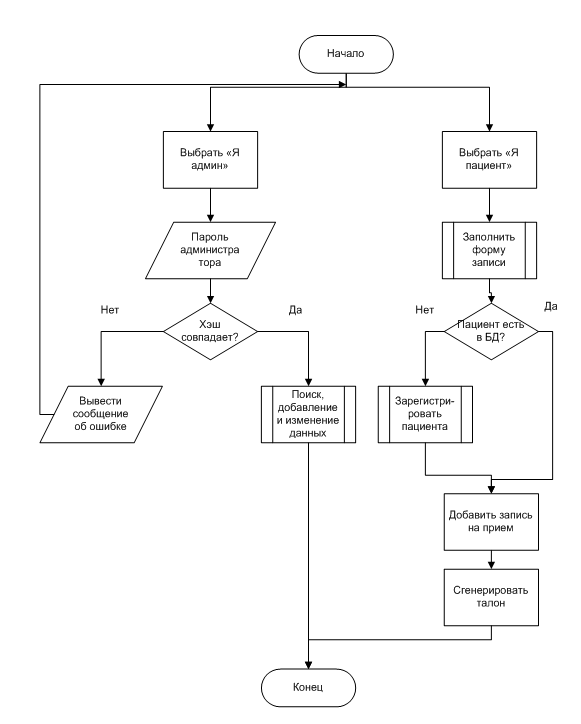
\includegraphics[width=0.8\linewidth]{block}}
\caption{Блок-схема алгоритма работы программы}
\label{block:block}
\end{figure}

\subsubsection{Численность, функции и квалификация персонала}

Для использования системы необходим администратор, который будет добавлять новых сотрудников и менять расписание уже добавленных, следить за целостностью системы, удалять ПДн пациентов по мере необходимости.

\subsubsection{Обеспечение потребительских характеристик системы}

Надежность обеспечивается путем следования стандартам написания кода и использования блоков try-catch для обработки исключительных ситуаций.
Производительность системы обеспечивается путем использования оптимальных алгоритмов.

\subsubsection{Функции, выполняемые системой}

Функциями, выполняемыми программой <<hospital\_register>>, являются регистрация пациентов, добавление записей на прием, печать талонов, управление расписанием и номенклатурой сотрудников (врачей), а также управление записями в БД. 

\subsubsection{Комплекс технических средств}

Для функционирования системы необходимы следующие аппаратные средства:

\begin{itemize}
  \item ОС Linux Ubuntu/Debian;
  \item процессор x86-архитектуры;
  \item объем ОЗУ для выполнения программы: не менее 300 Мб;
  \item объём видеопамяти: не менее 300 Мб;
  \item память на жестком диске: не менее 100 Мб для файлов БД и программы;
  \item монитор с разрешением 800x600 или выше;
  \item мышь, клавиатура;
  \item устройство для чтения CD;
  \item принтер.
\end{itemize}

\subsubsection{Информационное обеспечение системы}

Система поставляется с руководством пользователя и программиста.

\subsubsection{Программное обеспечение системы}

Система разворачивается на компьютере с ОС Linux Ubuntu/Debian.

\section{Мероприятия по подготовке персонала}

Провести ознакомление персонала с руководством пользователя.






